\begin{figure}[!htbp]\centering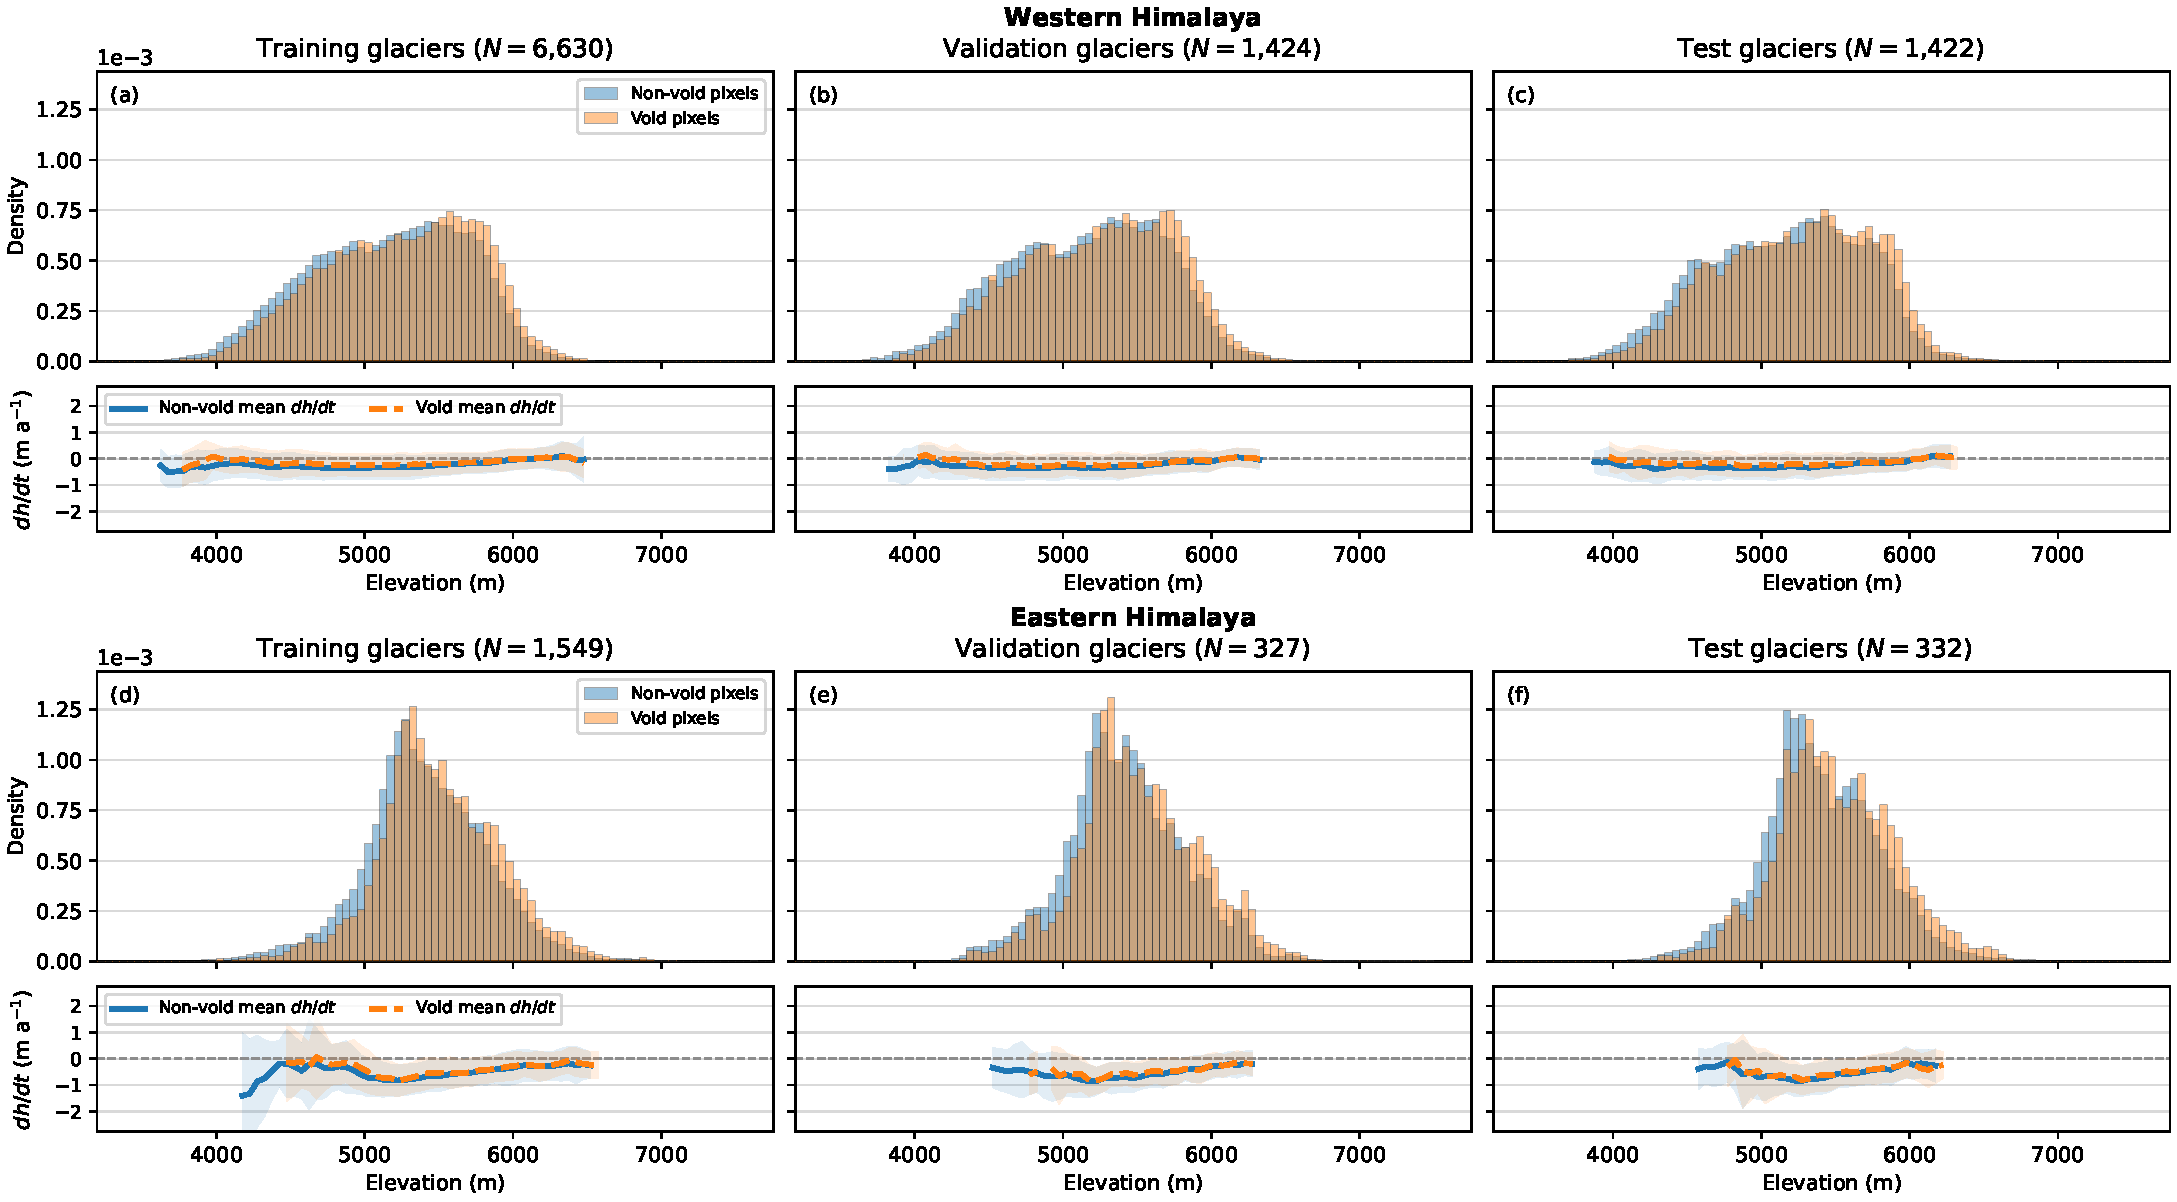
\includegraphics[width=\textwidth,height=.62\textheight,keepaspectratio]{fig02_distributions.pdf}\caption{Observed and withheld reference data in the Western (a–c) and Eastern (d–f) Himalaya, with columns showing training, validation, and test glaciers. Each lettered panel contains an elevation-density histogram above and elevation-change rates below. Blue denotes non-void pixels available to the methods, and orange denotes withheld void pixels. Histograms use 50 m elevation bins. Curves show bin-mean reference elevation-change rates for 2000–2018, with shading indicating within-bin standard deviations. Glaciers receive equal total weight, with equal weights for realizations and then finite pixels within each realization. Membership is defined separately for each mask. Training and validation panels show all 8,179 and 1,751 assigned glaciers. Test panels show the 1,754 evaluated test glaciers, excluding RGI60-14.17287. All panels share one elevation range spanning every finite reference pixel, from 3,195 to 7,755 m.}\label{fig:distributions}\end{figure}
